% ============================================================
% PHẦN B - PHƯƠNG PHÁP VÀ THỰC NGHIỆM CỦA SCIMKG (bài chỉ báo cáo)
%   Mỗi phần đánh số mục lại từ I. Phần B có 5 mục:
%   I Giới thiệu (B_intro), II Công trình liên quan (B_related),
%   III Phương pháp và IV Thực nghiệm (file này), V Kết luận (B_conclusion)
%   IV gồm: A kết quả công bố (mốc tham chiếu), B thiết lập, C Ex01 (chi phí một bài),
%   D Ex02 (kiểm chứng theo số vòng), E Ex03 (tìm đúng đoạn bài giảng),
%   F thảo luận và giới hạn
%   Bảng Phần B tạm gỡ nằm ở B_tables_parked.tex; mọi bảng số đo sinh bằng
%   report/tools/make_ex_tables.py vào report/tables/ (không sửa tay)
% ============================================================

% ------------------------------------------------------------
\section{Phương pháp}\label{sec:sm-method}
% ------------------------------------------------------------
\subsection{Tổng quan}\label{sec:sm-overview}
\SM{} nhận đầu vào là tài nguyên của các khóa học trực tuyến mở, gồm video bài giảng, slide, bài tập và chuẩn chương trình của môn học (Hình~\ref{fig:sm-pipeline}a).
Bài báo chọn ba môn khoa học tự nhiên bậc phổ thông của Trung Quốc là sinh học, vật lý và hóa học, vì các môn này giàu nội dung trực quan hơn những môn còn lại.
Đầu ra là một EKG đa phương thức tổ chức theo ba tầng: môn học, điểm kiến thức và khái niệm.
Mỗi khái niệm được gắn với lời giải thích bằng văn bản, ảnh minh họa, đoạn video nơi khái niệm được giảng và âm thanh đọc lời giải thích.

Về hình thức, bài toán gồm hai bài toán con nối tiếp nhau.
Bài toán thứ nhất là trích xuất khái niệm: cho tập đoạn văn $P=\{p_1,\dots,p_n\}$ lấy từ phụ đề video, mỗi đoạn gắn với một khoảng thời gian, tìm tập $C=\{c_1,\dots,c_m\}$ gồm những khái niệm thực sự thuộc môn $d$.
Chẳng hạn ``mô biểu bì'' và ``tế bào cơ'' là khái niệm sinh học, còn ``hệ thống'' quá chung chung và ``kính hiển vi'' chỉ là dụng cụ.
Bài toán thứ hai là căn chỉnh đa phương thức: với mỗi phương thức $m\in M=\{\text{văn bản},\text{ảnh},\text{video},\text{âm thanh}\}$, gán từng tài nguyên thuộc phương thức $m$ vào đúng khái niệm trong $C$.
Lấy khái niệm \emph{mô biểu bì} làm ví dụ, nó có một câu giải thích, các ảnh slide minh họa, đoạn video 07:52--10:24 nơi khái niệm được giảng và một tệp âm thanh đọc lời giải thích, rồi được nối với điểm kiến thức ``các cấp tổ chức của cơ thể động vật'' thuộc môn sinh học.

Luồng xử lý (Hình~\ref{fig:sm-pipeline}) gồm bốn thành phần nối tiếp.
Tiền xử lý biến video và slide thành các đoạn văn có mốc thời gian, các đoạn video và các ảnh.
Trích xuất khái niệm chạy chuỗi EVIA (Extraction, Verification, Integration, Augmentation) trên từng đoạn văn để ra tập $C$.
Căn chỉnh đa phương thức gắn ảnh, video và âm thanh vào từng khái niệm.
Cuối cùng, khái niệm và tài nguyên đi kèm được tổ chức và lưu thành JSON và RDF, phục vụ các ứng dụng như sinh câu hỏi đa phương thức, hỏi đáp, truy hồi chéo phương thức và trợ lý học tập.

Điểm đáng chú ý là \SM{} không huấn luyện hay tinh chỉnh trọng số của bất kỳ mô hình nào: mọi bước cần ``hiểu'' nội dung đều gọi mô hình có sẵn qua API với prompt soạn trước.
Phần gần với việc ``học'' nhất là vòng Self-Refine ở bước kiểm chứng, nơi mô hình nhận lại phản hồi của chính nó để sửa danh sách khái niệm, nhưng toàn bộ diễn ra lúc suy luận và không có gradient.
Tham số giải mã được cố định để giảm ngẫu nhiên: nhiệt độ 0, top-$p$ 0,1, frequency penalty 0,5, độ dài tối đa 1000 token và seed 42.
Riêng thí nghiệm theo kích thước mô hình dùng các LLM mở cỡ nhỏ (Qwen3, Gemma3, Phi-3), chạy cục bộ trên một GPU RTX 3090, cũng chỉ ở chế độ suy luận.

\begin{figure*}[t]
\centering
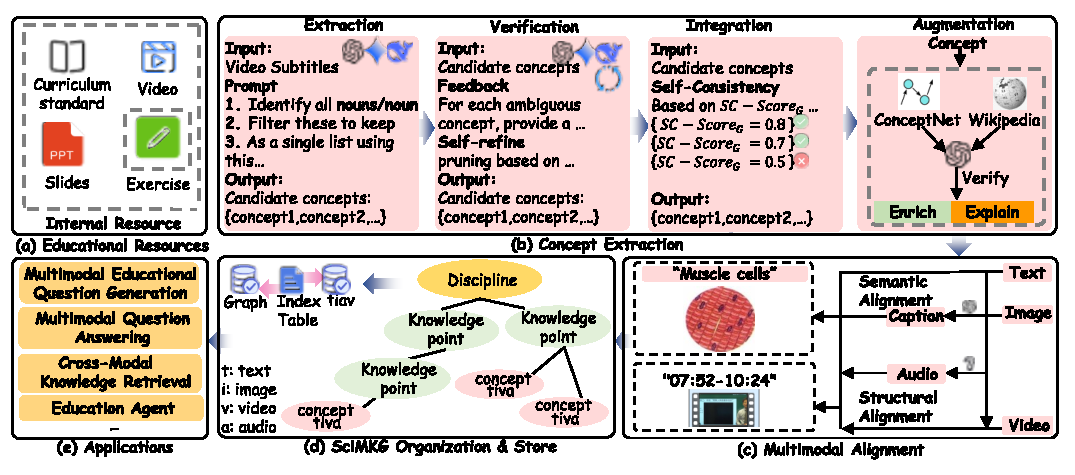
\includegraphics[width=\textwidth]{figures/fig_sm_overview_paper.pdf}
\caption{Khung xây dựng \SM{} (Hình 2 trong~\cite{lu2026scimkg}, giữ nguyên nhãn tiếng Anh của tác giả). \textbf{(a)} Tài nguyên giáo dục đầu vào: chuẩn chương trình, video, slide và bài tập. \textbf{(b)} Trích xuất khái niệm bằng chuỗi EVIA (Extraction, Verification, Integration, Augmentation). \textbf{(c)} Căn chỉnh đa phương thức: căn chỉnh ngữ nghĩa cho ảnh qua mô tả, căn chỉnh cấu trúc cho video và âm thanh. \textbf{(d)} Tổ chức và lưu trữ theo ba tầng môn học, điểm kiến thức và khái niệm. \textbf{(e)} Các ứng dụng của đồ thị.}
\label{fig:sm-pipeline}
\end{figure*}

\subsection{Thu thập và tiền xử lý}\label{sec:sm-preprocess}
Dữ liệu nguồn là video, slide và bài tập của các khóa học trực tuyến mở, kèm chuẩn chương trình.
Phụ đề của video được trích thành văn bản để tìm khái niệm, còn ảnh được tách từ slide để bổ sung phương thức cho khái niệm.
Để lời giảng rõ ràng và dễ tiếp cận hơn, bài báo dùng MLLM viết lại văn bản đã trích, sinh âm thanh tương ứng và ghi lại URL của từng video gốc.
Theo mã nguồn, văn bản là kết quả nhận dạng giọng nói (bước này làm thủ công, nằm ngoài mã; xem Mục~\ref{sec:sm-mismatch}).
Gemini gộp văn bản đó theo ngữ nghĩa thành các đoạn có mốc thời gian, và video được cắt thành các clip theo mốc đó.
Toàn bộ văn bản là tiếng Trung giản thể.

\subsection{Trích xuất khái niệm: chuỗi EVIA}\label{sec:sm-evia}
Chuỗi EVIA đã nêu ở phần tổng quan chạy trên từng đoạn phụ đề theo bốn bước.
Đầu vào của bước trích xuất (E) là văn bản của một đoạn; LLM xác định mọi danh từ và cụm danh từ rồi giữ lại những cụm thuộc môn học, và đầu ra là tập khái niệm ứng viên của đoạn.
Chẳng hạn, từ một đoạn nói về mô biểu bì, ứng viên có thể gồm ``mô biểu bì'', ``tế bào cơ'', ``hệ thống'', ``kính hiển vi'' và ``cơ quan'' (ví dụ minh họa của nhóm, không phải dữ liệu của bài).

Bước kiểm chứng (V) nhận tập ứng viên đó và trả về chính tập ấy kèm một điểm phiếu cho từng ứng viên.
Mỗi LLM trong ba LLM chạy năm vòng Self-Refine~\cite{madaan2023selfrefine}.
Ở mỗi vòng, LLM tự kiểm tra từng ứng viên có thuộc môn học hay không và nêu lý do ngắn cho ứng viên có thể bị loại (phản hồi), rồi lọc lại danh sách dựa trên các phản hồi đã tích lũy (sửa).
Ứng viên còn lại sau bước sửa được cộng một phiếu, nên điểm tối đa là 15.

Bước tích hợp (I) gộp các phiếu theo tinh thần Self-Consistency~\cite{wang2023selfconsistency}: ứng viên được nhiều mô hình và nhiều vòng giữ lại thì đáng tin hơn.
Ứng viên được giữ khi điểm tổng hợp đạt ngưỡng $\alpha=0{,}7$, mà bài mô tả là tần suất ứng viên được nhận ở bước kiểm chứng; nhóm hiểu đó là tỉ lệ phiếu trên số phiếu tối đa, tức ít nhất 11 trên 15 phiếu.
Trong ví dụ, ``mô biểu bì'' (15 phiếu), ``tế bào cơ'' (14) và ``cơ quan'' (11) được giữ, còn ``hệ thống'' và ``kính hiển vi'' (3 phiếu) bị loại.
Theo bài, Self-Refine làm sạch danh sách nên precision tăng, còn dùng nhiều LLM giúp không bỏ sót nên recall tăng; Mục~\ref{sec:sm-exp-pub} đối chiếu cách giải thích này với số liệu ablation, và Mục~\ref{sec:sm-ex02} kiểm tra lại tác động của kiểm chứng trên nhãn công bố.

Bước bổ sung (A) nhận tập khái niệm của I và trả về tập mở rộng cùng lời giải thích cho từng khái niệm, vì phụ đề chỉ chứa những gì giáo viên nói ra.
Mỗi khái niệm được tra trên ConceptNet để lấy các khái niệm lân cận theo tám quan hệ (IsA, RelatedTo, HasContext, PartOf, DefinedAs, Synonym, DerivedFrom, HasPrerequisite), qua các luật biểu thức chính quy do tác giả thiết kế; LLM sau đó lọc và kiểm tra chéo để chỉ giữ khái niệm thuộc môn học.
Các khái niệm này được liên kết với Wikipedia để lấy mô tả chi tiết, và LLM tóm tắt thành một câu giải thích ngắn gọn; bài báo coi việc bám Wikipedia là cách giảm ảo giác.

\subsection{Căn chỉnh đa phương thức}\label{sec:sm-align}
Căn chỉnh gắn từng phương thức vào khái niệm đã trích, nhờ khả năng hiểu liên phương thức của các MLLM.
Với ảnh, một MLLM ánh xạ mỗi ảnh vào khái niệm tương ứng bằng cách sinh mô tả ngữ nghĩa, rồi một MLLM khác kiểm tra cặp đó bằng cách chấm độ tin cậy dựa trên văn bản; chỉ những cặp có độ tin cậy trên 0,8 được giữ.
Với video, mỗi đoạn video được gắn với các khái niệm cùng xuất hiện trong đoạn đó, dựa trên ngữ nghĩa của văn bản khái niệm kết hợp với cấu trúc thời gian từ mốc thời gian, kèm URL để truy cập video gốc.
Với âm thanh, lời giải thích của khái niệm được viết lại dựa trên tri thức Wikipedia để giảm ảo giác, rồi chuyển thành âm thanh bằng TTS.

\subsection{Tổ chức và lưu trữ}\label{sec:sm-store}
\SM{} có ba tầng: tầng môn học ở trên cùng gồm sinh học, vật lý và hóa học; tầng điểm kiến thức ở giữa, tổ chức theo chuẩn chương trình và đề cương của các khóa MOOC; tầng khái niệm ở dưới cùng, chứa mọi khái niệm đa phương thức.
Môn học, điểm kiến thức, bài tập và khái niệm đa phương thức đều có mã định danh riêng và được liên kết thành một đồ thị phân cấp qua cơ chế tham chiếu chéo, lưu trong các bảng tham chiếu dạng JSON; đồ thị còn được xuất sang RDF tuân thủ IRI để dễ tái sử dụng.

Mỗi khái niệm và mỗi dữ liệu đa phương thức là một thực thể riêng, nối với nhau bằng mười một loại quan hệ: giải thích, ảnh, video và âm thanh (mỗi loại có một cặp quan hệ thuận và nghịch với khái niệm), quan hệ ``related to'' nối khái niệm với điểm kiến thức, và cặp quan hệ nối bài tập với điểm kiến thức.
Tổng cộng đồ thị có 1.356 điểm kiến thức, 34.630 khái niệm, 403.400 bộ ba, 763 bài tập, 10.527 ảnh, 10.425 video và 34.630 tệp âm thanh; ảnh phủ 39\% khái niệm, video phủ 80\% và âm thanh phủ 100\%.

\subsection{Bổ sung từ mã nguồn và điểm không khớp với bài báo}\label{sec:sm-mismatch}
Bài báo chỉ mô tả ở mức khái quát, nên nhóm đối chiếu với mã công bố~\cite{kgbnu2026scimkgcode}.
Các điểm đáng chú ý:
\begin{itemize}
\item \textbf{Tiền xử lý.} Nhận dạng giọng nói làm thủ công, ngoài mã; việc gộp đoạn bằng Gemini, cắt clip và tách ảnh nằm ở các hàm và dịch vụ ngoài rời nhau, phần điều phối chỉ còn ở dạng dòng chú thích. Phát biểu cuối của mỗi tài liệu bị bỏ.
\item \textbf{Trích xuất (E).} Chỉ gọi DeepSeek-V3, không phải nhiều LLM như bài mô tả. Một danh sách khái niệm đã gặp dùng chung cho toàn bộ dữ liệu, nên khái niệm chỉ gắn với lần giảng đầu tiên (mốc thời gian và clip).
\item \textbf{Kiểm chứng (V).} Prompt nhắm vào thuật ngữ mơ hồ liên ngành và dụng cụ thí nghiệm; mỗi vòng sửa luôn xuất phát từ danh sách ban đầu, nên giống lấy mẫu lặp hơn là sửa dần.
\item \textbf{Tích hợp (I).} Hệ số chuẩn hóa bằng 1 và điểm khởi tạo là 1, nên điều kiện ngưỡng 0,7 luôn đúng và, theo cách nhóm đọc mã, mọi ứng viên đều được giữ. Đây là nhận xét về mã công bố, không phải về cách dữ liệu công bố được sinh ra.
\item \textbf{Bổ sung (A).} Bộ luật cho ConceptNet để trống; khái niệm được dịch bằng Baidu Translate để tra Wikipedia; nhánh ``không tìm thấy trang'' không bao giờ chạy vì lỗi kiểu dữ liệu.
\item \textbf{Căn chỉnh.} Ảnh: GPT-4o gọi ba lần rồi lấy hợp, không có MLLM thứ hai và ngưỡng 0,8; ảnh còn bổ sung khái niệm mới. Video: mã trong repo chỉ cắt clip; bước dựng bộ ba có đọc trường URL video của từng khái niệm, nhưng không có mã nào tạo trường này. Gói \texttt{scimkg} 0.1.1 trên TestPyPI có ghép khái niệm với clip theo mốc thời gian, nhưng chỉ trả kết quả cho trang web minh họa, không đưa vào bộ ba hay RDF. Âm thanh: mô hình tts-1 của OpenAI.
\item \textbf{Lưu trữ.} Mỗi khái niệm sinh ít nhất 6 bộ ba theo cặp thuận-nghịch, thêm 2 cho mỗi liên kết khái niệm-ảnh và 2 cho mỗi liên kết khái niệm-video, nên tổng hơn 400 nghìn bộ ba; số liên kết lớn hơn số ảnh (10.527) vì một ảnh có thể gắn với nhiều khái niệm; ánh xạ RDF của video dùng khóa ``an video'', khác nhãn ``a video'' lúc sinh bộ ba.
\end{itemize}

% ------------------------------------------------------------
\section{Thực nghiệm}\label{sec:sm-exp}
% ------------------------------------------------------------
Bài báo đo chất lượng trích xuất và căn chỉnh nhưng không nêu chi phí chạy: toàn văn không có số token, giá hay tiền nào.
Với một đồ thị phủ hơn một nghìn điểm kiến thức, đây lại là điều người muốn áp dụng cần biết trước.
Phần này trả lời ba câu hỏi: (1) dựng một bài học tốn bao nhiêu lời gọi và token; (2) kiểm chứng đổi được bao nhiêu chất lượng với chi phí thêm bao nhiêu; (3) chỉ mục theo khái niệm của đồ thị tìm đúng đoạn bài giảng tốt đến đâu so với mốc ngẫu nhiên và mốc chỉ dùng văn bản.
Với câu (1), nhóm đo bằng số lượt gọi và số token, vì tiền phụ thuộc mô hình và bảng giá thay đổi theo thời điểm; tiền chỉ được quy đổi cho gpt-6-luna, mô hình đã dùng.
Ex01 (Mục~\ref{sec:sm-ex01}) trả lời câu (1) cho một bài học.
Ex02 (Mục~\ref{sec:sm-ex02}) đổi số vòng kiểm chứng để trả lời câu (2).
Ex03 (Mục~\ref{sec:sm-ex03}) trả lời câu (3) trên cùng sáu bài.
Trừ Mục~\ref{sec:sm-exp-pub}, mọi số đo ở đây đến từ bộ chạy của nhóm (Mục~\ref{sec:sm-exp-setup}).

\subsection{Kết quả công bố làm mốc tham chiếu}\label{sec:sm-exp-pub}
Bảng~\ref{tab:sm-pub} lấy lại kết quả trích xuất khái niệm của bài trên tập đánh giá gồm 100 bài học và 4.479 khái niệm; các baseline dựa trên LLM đều dùng GPT-4o.
Phương pháp đầy đủ đạt F1 cao nhất, 0,803.
Các dòng ``EVIA w/o \dots'' là phần cắt bỏ: ``MLs'' là nhiều LLM, còn ``SF-FD'' là vòng tự phản hồi.
Bài còn quét số vòng lặp và ngưỡng trên chín tổ hợp; cấu hình 5 vòng, ngưỡng 0,7 cho F1 tốt nhất.
Về căn chỉnh ảnh, bài nêu bốn điểm tự động (CLIP 0,83, BLIP-ITM 0,76, X-VLM-ITM 0,81, VQAScore 0,75) và điểm trung bình 0,73 của năm chuyên gia; căn chỉnh video và âm thanh không được đo.

\begin{table}[t]
\centering
\caption{Trích xuất khái niệm theo bài báo (chọn lọc).}
\label{tab:sm-pub}
\small
\setlength{\tabcolsep}{4pt}
\resizebox{\columnwidth}{!}{%
\begin{tabular}{@{}lcccc@{}}
\toprule
Phương pháp & P & R & F1 & MCC \\
\midrule
Decomposed-QA & 0,935 & 0,570 & 0,712 & \textbf{0,741} \\
GPT-NER & 0,530 & \textbf{0,931} & 0,681 & 0,621 \\
LinkNER & 0,855 & 0,644 & 0,734 & 0,732 \\
UniversalNER & 0,873 & 0,617 & 0,718 & 0,722 \\
\midrule
EVIA, Qwen3-14B+Gemma3-27B+Phi-3-14B & 0,879 & 0,637 & 0,739 & 0,730 \\
EVIA w/o MLs$^{a}$ & 0,769 & 0,342 & 0,477 & 0,509 \\
EVIA w/o SF-FD & 0,374 & 0,589 & 0,459 & 0,428 \\
EVIA w/o MLs + SF-FD$^{b}$ & 0,340 & 0,290 & 0,312 & 0,315 \\
\textbf{EVIA (đầy đủ)} & \textbf{0,947} & 0,702 & \textbf{0,803} & 0,729 \\
\bottomrule
\end{tabular}}
\par\smallskip
{\footnotesize\raggedright $^{a}$Một mô hình, có vòng tự phản hồi: gần cấu hình đầy đủ của Ex02. $^{b}$Một mô hình, dùng thẳng kết quả trích xuất: gần cấu hình tắt kiểm chứng của Ex02.\par}
\end{table}

Nhóm dùng các số này làm mốc về hướng, không làm mốc về giá trị.
Bài chạy nhiều LLM thương mại trên 100 bài, còn Ex02 chạy một mô hình trên sáu bài.
Theo hai dòng này, vòng tự phản hồi nâng F1 từ 0,312 lên 0,477, chủ yếu nhờ precision (từ 0,340 lên 0,769).
Hai dòng ``EVIA w/o MLs'' và ``EVIA (đầy đủ)'' cho thấy dùng nhiều LLM nâng recall từ 0,342 lên 0,702, đúng như bài giải thích, nhưng precision cũng tăng từ 0,769 lên 0,947; vậy nhiều LLM không chỉ giúp bớt bỏ sót mà còn lọc bớt ứng viên sai.

\subsection{Thiết lập thực nghiệm}\label{sec:sm-exp-setup}
\textbf{Dữ liệu.}
Nhóm lấy sáu bài từ bộ MOOC mà tác giả công bố, mỗi môn (sinh học, vật lý, hóa học) hai bài (Bảng~\ref{tab:sm-lessons}); bộ này kèm tập nhãn khái niệm chuẩn (ground truth) theo từng bài, và nhóm dùng tập nhãn đó để chấm.
Văn bản đưa vào mô hình và nhãn dùng để chấm được tách riêng; nhãn không được đọc hay gửi đi trong quy trình dựng đồ thị.
Văn bản bài giảng bằng tiếng Trung được giữ nguyên, chỉ tên bài ghi bằng tiếng Việt.
Bộ công bố có văn bản và ảnh nhưng không có video và PDF gốc, nên ba thực nghiệm này không dùng video.
Ex01 dùng 27 ảnh slide của bài Cấu tạo hệ thần kinh; Ex02 và Ex03 chỉ dùng văn bản.

\begin{table}[t]
\centering
\caption{Sáu bài dùng trong thực nghiệm (bộ MOOC do tác giả công bố).}
\label{tab:sm-lessons}
\small
\begin{tabular}{@{}llrr@{}}
\toprule
Bài & Môn & Đoạn & Nhãn \\
\midrule
Cấu tạo hệ thần kinh & Sinh học & 14 & 30 \\
Sinh sản của động vật lưỡng cư & Sinh học & 7 & 57 \\
Áp suất khí quyển & Vật lý & 12 & 21 \\
Lực đẩy & Vật lý & 14 & 19 \\
Axit sunfuric và muối sunfat & Hóa học & 15 & 13 \\
Protein & Hóa học & 13 & 48 \\
\midrule
\textbf{Tổng} & & \textbf{75} & \textbf{188} \\
\bottomrule
\end{tabular}
\end{table}

\textbf{Cấu hình và khác biệt so với bài.}
Trong cả ba thực nghiệm, mọi lời gọi LLM dùng một mô hình duy nhất là gpt-6-luna ở mức suy luận thấp, gọi qua công cụ dòng lệnh bằng tài khoản thuê bao, thay cho nhiều LLM của bài.
Nhóm giữ số vòng kiểm chứng bằng 5 và ngưỡng 0,7 như bài.
Điều kiện tích hợp trong mã công bố được nhóm đọc là luôn đúng, nên mọi ứng viên đều được giữ (Mục~\ref{sec:sm-mismatch}).
Bộ chạy của nhóm sửa điều này: điểm tích hợp là số phiếu của kiểm chứng chia cho số phiếu tối đa (số mô hình nhân số vòng), và ngưỡng 0,7 có tác dụng thật.
Với một mô hình, năm vòng cần ít nhất bốn phiếu (4 trên 5 là 0,8, đạt ngưỡng; 3 trên 5 là 0,6, không đạt), còn một vòng cần đúng một phiếu.
Các khác biệt còn lại: căn chỉnh ảnh không có ngưỡng 0,8 của bài báo; lời giải thích tra Wikipedia tiếng Trung bằng đúng tên khái niệm và lấy các đoạn văn dài từ 30 ký tự, thay cho bước dịch bằng Baidu Translate rồi tra Wikipedia của mã gốc, vì bước đó cần khóa dịch vụ và máy chủ trung gian (Mục~\ref{sec:sm-mismatch});tiền xử lý dùng văn bản và ảnh đã công bố thay cho bước thủ công của mã gốc; tập khái niệm đã gặp được đặt lại theo từng bài.
Bộ luật dựa trên sáu mẫu câu tiếng Anh của ConceptNet, bỏ Synonym và DerivedFrom, và khớp mọi thuật ngữ đã tra thay vì chỉ thuật ngữ cuối như mã gốc.
Vì API ConceptNet trả lỗi 502 khi chạy, truy vấn được trả lời từ bản dump 5.7.0 đã công bố, đọc thành cùng cấu trúc dữ liệu mà mã gốc đọc từ API.

\subsection{Ex01: chi phí một bài học}\label{sec:sm-ex01}
Ex01 chạy trọn bài ``Cấu tạo hệ thần kinh'' (14 đoạn, 27 ảnh) từ văn bản đến đồ thị bằng một luồng duy nhất; Bảng~\ref{tab:sm-ex01-cost} tách số đo theo từng bước.

\textbf{Cách đo chi phí.}
Các lượt chạy dùng tài khoản thuê bao nên không có hóa đơn theo token.
Vì vậy nhóm đếm token theo hai cách và dùng hai số đó để ước lượng tiền, một số cao và một số thấp.
Cách thứ nhất lấy số do công cụ dòng lệnh báo, gọi là token CLI.
Số này lớn, nhiều khả năng vì công cụ gửi kèm một phần nội dung cố định của nó trong mỗi lượt (xem nhận xét 3 bên dưới).
Công cụ cũng cho biết bao nhiêu token đầu vào là phần lặp lại của lượt trước; nhà cung cấp giữ sẵn phần này (cached input) nên tính giá rẻ hơn.
Cách thứ hai chỉ đếm nội dung do nhóm soạn: prompt, schema và ảnh, gọi là token kiểu API.
Chữ được đếm bằng bộ tách từ \texttt{o200k\_base}, còn ảnh được ước lượng theo quy tắc tính token ảnh của OpenAI.
Số này nhỏ hơn token CLI vì không có phần nội dung cố định.
Cách này không biết phần nào được lưu sẵn, nên nhóm tính mọi token vào theo giá thường.
Số lượt gọi và số token ra giống nhau ở cả hai cách.
Token CLI cho số tiền cao (cận trên), token kiểu API cho số tiền thấp (cận dưới).
Ex01 có cả hai (Bảng~\ref{tab:sm-ex01-cost}); Ex02 chỉ in token kiểu API nên chỉ có cận dưới.
Mọi lượt gọi trong Ex01 và Ex02 đều có số token; lượt nào dùng lại kết quả đã lưu cục bộ thì không gửi yêu cầu mới và không được tính thêm.


Quy ra tiền dùng giá nhập, giá nhập đã lưu sẵn và giá xuất của mô hình, tính cho một triệu token: token vào chưa lưu sẵn nhân giá nhập, cộng token vào đã lưu sẵn nhân giá nhập đã lưu sẵn, cộng token ra nhân giá xuất.
Với gpt-6-luna (giá nhập 0,10 USD, giá nhập đã lưu sẵn 0,01 USD, giá xuất 0,50 USD), cận dưới 0,027 USD dùng token kiểu API và coi mọi token vào là chưa lưu sẵn; cận trên 0,19 USD dùng token CLI.
Hai cận này chưa thật chặt.
Nếu một phần đầu vào được lưu sẵn, chi phí thấp hơn cận dưới tối đa khoảng 0,018 USD.
Cận trên không tính phụ phí ghi vào bộ nhớ đệm, vì công cụ dòng lệnh không báo số token ghi; nếu tính mọi token vào chưa lưu sẵn theo giá ghi 0,125 USD mỗi triệu token, cận trên lên khoảng 0,23 USD.

% Bảng sinh tự động từ số đo bằng report/tools/make_ex_tables.py; không sửa tay.
\begin{table*}[t]
\centering
\caption{Chi phí Ex01 theo bước, lượt gpt-6-luna trên bài ``Cấu tạo hệ thần kinh''. Token vào CLI gồm ngữ cảnh cố định của công cụ; token vào kiểu API là số đếm trên prompt và schema, cộng token ảnh ước lượng. Chưa gồm tiền xử lý và ghép, cắt video (không đo được vì thiếu video và PDF gốc); tạo âm thanh chạy cục bộ nên không có lượt gọi.}
\label{tab:sm-ex01-cost}
\small
\setlength{\tabcolsep}{3pt}
% Generated by report/tools/make_ex_tables.py from measured run files; do not edit by hand.
\begin{tabular}{@{}lrrrrrrr@{}}
\toprule
Bước & Lượt gọi & \begin{tabular}[c]{@{}r@{}}Token vào,\\CLI\end{tabular} & \begin{tabular}[c]{@{}r@{}}trong đó\\đã lưu sẵn\end{tabular} & \begin{tabular}[c]{@{}r@{}}Token vào,\\kiểu API\end{tabular} & Token ra & \begin{tabular}[c]{@{}r@{}}Tỉ lệ\\tổng token\end{tabular} & Thời gian (phút) \\
\midrule
Trích xuất (E) & 14 & 176.344 & 48.128 & 3.532 & 676 & 4,1\% & 1,2 \\
Kiểm chứng (V) & 120 & 1.525.309 & 986.624 & 43.995 & 6.298 & 35,3\% & 10,3 \\
Tích hợp (I) & 0 & 0 & 0 & 0 & 0 & 0,0\% & 0,0 \\
Bổ sung (A) và truy hồi nguồn & 16 & 201.026 & 84.224 & 3.548 & 699 & 4,6\% & 1,3 \\
Tạo giải thích & 104 & 1.351.503 & 950.528 & 67.559 & 4.224 & 31,2\% & 10,7 \\
Căn chỉnh ảnh & 81 & 1.071.750 & 709.888 & 76.215 & 3.012 & 24,8\% & 7,7 \\
Tạo âm thanh (cục bộ) & 0 & 0 & 0 & 0 & 0 & 0,0\% & 0,6 \\
\midrule
\textbf{Tổng} & \textbf{335} & \textbf{4.325.932} & \textbf{2.779.392} & \textbf{194.849} & \textbf{14.909} & \textbf{100\%} & \textbf{31,8} \\
\bottomrule
\end{tabular}

\end{table*}

Đầu ra gồm 38 khái niệm sau kiểm chứng và tích hợp; bước bổ sung từ ConceptNet thêm 64 khái niệm và căn chỉnh ảnh thêm 2, thành 104 khái niệm cuối.
Mỗi khái niệm cuối có một giải thích: 82 có văn bản Wikipedia tiếng Trung dùng được, còn 22 khái niệm không có trang trùng tên (lỗi 404) nên dùng giải thích dự phòng của mô hình và được gắn nhãn không có nguồn.
Văn bản nguồn của 23 giải thích chưa nằm trong Bảng~\ref{tab:sm-ex01-cost}; phần này làm tổng token vào chênh dưới 1\%.
Đồ thị gồm 744 bộ ba, tương ứng 1.097 câu lệnh RDF, kèm 104 tệp âm thanh (tổng khoảng 733 giây).

Bảng~\ref{tab:sm-ex01-cost} cho ba nhận xét.
\begin{enumerate}
\item Ba bước kiểm chứng, tạo giải thích và căn chỉnh ảnh chiếm khoảng 91\% token CLI. Kiểm chứng gọi mô hình 120 lần: mỗi vòng có hai lượt (phản hồi rồi sửa), năm vòng là 10 lượt cho một đoạn, và chỉ 12 trong 14 đoạn được kiểm chứng. Hai đoạn còn lại (đoạn 9 và 12) không còn ứng viên, vì mọi khái niệm trích được ở đó đã xuất hiện ở đoạn trước, mà mã chỉ giữ lần xuất hiện đầu tiên và bỏ qua kiểm chứng khi đoạn rỗng. Tích hợp và xuất đồ thị chạy bằng mã nên không có lượt gọi.
\item Bước bổ sung từ ConceptNet tốn ít token nhưng thêm 64 khái niệm, nhiều hơn số còn lại sau kiểm chứng. Đây là số khái niệm được thêm, chưa phải số khái niệm đúng: Ex02 chấm ngay sau bước tích hợp, trước khi bổ sung, và nhãn của tác giả chỉ gồm khái niệm có trong bài nên không chấm được phần bổ sung (không khái niệm nào trùng hẳn nhãn).
\item Mỗi lượt có khoảng 12.560 đến 13.230 token vào CLI, trong khi mỗi giải thích chỉ trả về khoảng 41 token ra. Ở các bước chỉ có chữ, token kiểu API chỉ chiếm khoảng 2 đến 5\% token CLI; ở bước căn chỉnh ảnh, token kiểu API (gồm cả token ảnh ước lượng) chiếm khoảng 7\%, trong đó phần chữ khoảng 4\%. Phần chênh là ngữ cảnh cố định mà công cụ tự thêm vào mỗi lượt: ở 254 lượt chỉ có chữ, token vào CLI trừ đi token của prompt và schema luôn nằm trong khoảng 12.339 đến 12.350, dù prompt dài từ 127 đến 3.457 token. Tính cho cả 335 lượt, phần cố định này khoảng 4,14 triệu token, tức khoảng 96\% token vào CLI.
\end{enumerate}

Đếm theo kiểu API, tổng token vào là 194.849, trong đó 30.855 là token ảnh ước lượng (mỗi ảnh được gửi ba lần) và 163.994 là văn bản; tổng này bằng khoảng 4,5\% token vào CLI.
Nếu phần cố định ở lượt có ảnh cũng như ở lượt chỉ có chữ, token ảnh suy từ số CLI là khoảng 26.400, thấp hơn ước lượng khoảng 14\%, nên số ước lượng hơi cao.
Hai cách đếm cho cận dưới và cận trên khác nhau khoảng 7 lần ở gpt-6-luna (0,027 so với 0,19 USD), nhỏ hơn nhiều so với tỉ lệ khoảng 22 lần giữa hai cách đếm token vào (194.849 so với 4.325.932 token).
Khoảng cách hẹp lại vì hai lý do: khoảng 64\% token vào CLI được tính theo giá đã lưu sẵn, rẻ hơn giá bình thường, trong khi token vào kiểu API bị coi là chưa lưu sẵn toàn bộ; và token ra, giống nhau ở cả hai cách, chiếm một phần chi phí không đổi theo cách đếm token vào, nên kéo tỉ lệ chi phí lại gần hơn tỉ lệ token.
Báo cáo ghi cả hai cận thay vì chọn một.
Cận trên cao hơn thực tế vì gồm phần ngữ cảnh cố định của công cụ nói trên; cận dưới có thể thấp hơn thực tế, vì một chương trình gọi API thật có thể gửi thêm nội dung mà đếm này không có.
Tiền xử lý và ghép, cắt video không đo được vì nhóm không có video và PDF gốc của bài; các bước này có thể làm chi phí thực tế cao hơn.
\wandb{https://wandb.ai/nhinbm-hcmus/SciMKG/runs/7b20992d11ea}

\subsection{Ex02: kiểm chứng đổi được gì}\label{sec:sm-ex02}
Ex02 đo kiểm chứng (V) đổi được bao nhiêu chất lượng khái niệm.
Nhóm chọn V vì đây là bước tốn nhiều lời gọi và token CLI nhất ở Ex01: 120 trong 335 lượt gọi và 35,3\% tổng token CLI (Bảng~\ref{tab:sm-ex01-cost}).

\textbf{Thiết kế.}
Nhóm chỉ đổi số vòng kiểm chứng: 0 vòng, 1 vòng, và 5 vòng như bài báo; ở 0 vòng V không được gọi nên tập chấm chính là ứng viên của E.
Mô hình, tham số và cách dựng đầu vào giữ như Ex01.
Mỗi cấu hình chạy các bước E, V, I và A trên văn bản của sáu bài, không chạy ảnh và giải thích, nên chi phí chỉ gồm các bước này.
E được gọi lại ở mỗi cấu hình, nên ba cấu hình có ba lượt E khác nhau trên cùng đầu vào; riêng bài Cấu tạo hệ thần kinh ở 5 vòng dùng lại kết quả của Ex01.

\textbf{Cách chấm.}
Nhóm chấm ngay sau bước tích hợp (I), trên nhãn công bố: với mỗi bài, gộp khái niệm của mọi đoạn, loại trùng, rồi so với nhãn của đúng bài đó.
Bước bổ sung (A) không được chấm, vì phép chấm đặt trước A và nhãn chỉ gồm khái niệm có trong bài (nhận xét 2 ở Mục~\ref{sec:sm-ex01}).
Bỏ A không đổi precision, recall hay F1 nên nhóm không lập cấu hình tắt bổ sung; A vẫn chạy để Ex03 (Mục~\ref{sec:sm-ex03}) dùng lại ba đồ thị đầy đủ.
Nếu chấm cả phần bổ sung, recall chỉ tăng 0,005 đến 0,011 (mỗi cấu hình chỉ khớp thêm hai nhãn trên sáu bài), còn precision giảm từ khoảng 0,30--0,34 xuống 0,07--0,09 và F1 giảm khoảng 0,23 đến 0,26.
Vì nhãn chỉ gồm khái niệm có trong bài, số này cho thấy A chủ yếu thêm khái niệm ngoài bài, chưa cho biết chúng đúng hay sai.
Chỉ số chính là khớp đúng từng chuỗi sau chuẩn hóa NFKC và đổi phồn thể sang giản thể bằng OpenCC, cùng phép chuẩn hóa mà đường ống dùng để loại trùng ở bước gộp.
Khớp chuỗi con (một bên chứa bên kia, chuỗi ngắn có ít nhất hai ký tự) chỉ dùng để thăm dò.
Precision tính trên khái niệm dự đoán, recall tính trên nhãn; nhóm tính từng bài rồi lấy trung bình cộng sáu bài.
Mỗi lượt cũng ghi trần recall của E, tức recall của toàn bộ ứng viên trước khi V lọc.
Nhãn công bố có thể thiếu khái niệm đúng, và một dự đoán đúng nhưng không có trong nhãn vẫn bị tính sai; vì vậy precision đo được là cận dưới của precision thật, còn recall chỉ đo độ phủ trên nhãn đã có.

\begin{table}[t]
\centering
\caption{Ex02: trung bình sáu bài theo số vòng kiểm chứng. F1 là trung bình của F1 từng bài nên không bằng trung bình điều hòa của hai dòng đầu. Chi phí tính theo giá gpt-6-luna, chỉ cho E, V và A trên văn bản (không gồm ảnh và giải thích).}
\label{tab:sm-ex02-summary}
\footnotesize
\resizebox{\columnwidth}{!}{% Generated by report/tools/make_ex_tables.py from measured run files; do not edit by hand.
\begin{tabular}{@{}lccc@{}}
\toprule
Chỉ số (trung bình sáu bài) & 0 vòng & 1 vòng & 5 vòng \\
\midrule
Precision & 0,302 & 0,327 & 0,344 \\
Recall & 0,634 & 0,455 & 0,450 \\
F1 & 0,392 & 0,362 & 0,373 \\
F1 khớp chuỗi con (thăm dò) & 0,560 & 0,543 & 0,539 \\
Trần recall của E & 0,634 & 0,627 & 0,609 \\
Số lời gọi, sáu bài & 254 & 335 & 882 \\
Token vào, kiểu API & 73.829 & 102.910 & 330.238 \\
Token ra, kiểu API & 14.641 & 21.868 & 54.166 \\
Chi phí, USD (Luna, cận dưới) & 0,015 & 0,021 & 0,060 \\
Bài có F1 thấp hơn cấu hình 5 vòng & 2 / 6 & 4 / 6 & – \\
\bottomrule
\end{tabular}
}
\end{table}

\begin{table*}[t]
\centering
\caption{Ex02: precision (P), recall (R) và F1 từng bài theo số vòng kiểm chứng, khớp đúng sau chuẩn hóa. Mỗi ô là một lần chạy.}
\label{tab:sm-ex02-quality}
\footnotesize
\setlength{\tabcolsep}{4pt}
% Generated by report/tools/make_ex_tables.py from measured run files; do not edit by hand.
\begin{tabular}{@{}lccccccccc@{}}
\toprule
 & \multicolumn{3}{c}{0 vòng} & \multicolumn{3}{c}{1 vòng} & \multicolumn{3}{c}{5 vòng (đầy đủ)} \\
\cmidrule(lr){2-4}\cmidrule(lr){5-7}\cmidrule(l){8-10}
Bài & P & R & F1 & P & R & F1 & P & R & F1 \\
\midrule
Cấu tạo hệ thần kinh & 0,435 & 0,900 & 0,587 & 0,468 & 0,733 & 0,571 & 0,526 & 0,667 & 0,588 \\
Sinh sản của động vật lưỡng cư & 0,657 & 0,842 & 0,739 & 0,689 & 0,737 & 0,712 & 0,667 & 0,667 & 0,667 \\
Áp suất khí quyển & 0,167 & 0,333 & 0,222 & 0,286 & 0,191 & 0,229 & 0,250 & 0,191 & 0,216 \\
Lực đẩy & 0,118 & 0,316 & 0,171 & 0,067 & 0,105 & 0,082 & 0,120 & 0,158 & 0,136 \\
Axit sunfuric và muối sunfat & 0,132 & 0,769 & 0,225 & 0,107 & 0,462 & 0,174 & 0,132 & 0,538 & 0,212 \\
Protein & 0,301 & 0,646 & 0,411 & 0,343 & 0,500 & 0,407 & 0,371 & 0,479 & 0,418 \\
\midrule
\textbf{Trung bình} & \textbf{0,302} & \textbf{0,634} & \textbf{0,392} & \textbf{0,327} & \textbf{0,455} & \textbf{0,362} & \textbf{0,344} & \textbf{0,450} & \textbf{0,373} \\
\bottomrule
\end{tabular}

\end{table*}

Bảng~\ref{tab:sm-ex02-summary} và Bảng~\ref{tab:sm-ex02-quality} cho bốn nhận xét.
\begin{enumerate}
\item F1 thay đổi ít giữa ba cấu hình: 0,392 với 0 vòng, 0,362 với 1 vòng và 0,373 với 5 vòng. Trần recall của E dao động từ 0,609 đến 0,634 dù đầu vào giống nhau, vì E được gọi lại ở mỗi cấu hình; nhóm lấy mức 0,025 này làm ước lượng thô về độ nhiễu của một lần chạy. Chênh lệch F1 lớn nhất giữa các cấu hình (0,030) cùng cỡ mức đó, và mỗi ô chỉ có một lần chạy, nên nhóm chưa thể nói cấu hình nào tốt hơn.
\item Kiểm chứng làm recall giảm rõ nhưng chỉ nâng precision ít. Từ 0 vòng sang 5 vòng, recall giảm 0,184 (từ 0,634 xuống 0,450), lớn hơn nhiều mức nhiễu 0,025; precision tăng 0,042 (từ 0,302 lên 0,344), chỉ cùng cỡ mức nhiễu. Phần lớn thay đổi xảy ra ngay ở vòng đầu: từ 0 sang 1 vòng, recall giảm 0,179 và precision tăng 0,025; từ 1 sang 5 vòng, recall chỉ giảm thêm 0,005 và precision tăng thêm 0,017.
\item So với bài báo, precision đổi cùng chiều nhưng mức chênh khác nhiều, còn recall đổi ngược chiều. Trên một mô hình, bài báo cho thấy vòng tự phản hồi nâng precision từ 0,340 lên 0,769 và recall từ 0,290 lên 0,342 (Bảng~\ref{tab:sm-pub}, các dòng ``EVIA w/o MLs'' và ``EVIA w/o MLs + SF-FD''). Một giả thuyết là cấu hình 0 vòng của nhóm không lọc khái niệm nào, nên recall nền (0,634) cao hơn nhiều so với dòng tương ứng của bài; bài không mô tả đủ cách tạo dòng cắt bỏ này để kiểm tra giả thuyết đó.
\item Chất lượng không tăng theo chi phí. Năm vòng dùng 882 lời gọi, gấp 3,5 lần cấu hình 0 vòng (254 lời gọi), và chi phí kiểu API gấp khoảng bốn lần (0,060 so với 0,015 USD, theo giá gpt-6-luna). Mức tăng đến từ V: 700 lời gọi ở 5 vòng, tức 10 lời gọi cho mỗi đoạn có ứng viên (70 trong 75 đoạn), trong khi số lời gọi của A giảm từ 179 xuống 107. Chi phí tăng nhanh hơn số lời gọi vì lời gọi của V mang theo danh sách ứng viên và phản hồi các vòng trước, nên token vào kiểu API trung bình mỗi lời gọi tăng từ 291 lên 374.
\end{enumerate}

Trên sáu bài này, chưa thấy kiểm chứng làm tăng F1 trong khi nó làm chi phí tăng khoảng bốn lần.
Điều này chưa đủ để bỏ V, vì bài báo dùng ba mô hình khác nhau cho V, còn nhóm chỉ dùng một mô hình, sáu bài và một lần chạy cho mỗi ô.
\wandb{https://wandb.ai/nhinbm-hcmus/SciMKG/runs/ex02-8319b815}

\subsection{Ex03: tìm đúng đoạn bài giảng}\label{sec:sm-ex03}
Bài báo nói đồ thị gắn khái niệm với đoạn video để phục vụ truy hồi, nhưng không đo tác vụ nào.
Ex03 kiểm tra trên cùng sáu bài: cho một câu, đồ thị có chỉ ra đúng đoạn bài giảng chứa câu đó không.
Vì Ex02 không chạy căn chỉnh ảnh hay video, tác vụ này chỉ kiểm tra phần văn bản của đồ thị, chưa kiểm tra phần đa phương thức mà bài báo mô tả cho truy hồi.
Hỏi đáp trắc nghiệm bị loại vì các bộ có sẵn chỉ có từ 1 đến 38 câu khớp từ khóa mỗi bài.

\textbf{Truy vấn và đáp án.}
Nhóm tách bản ghi của sáu bài theo dấu câu, giữ các câu có ít nhất 15 ký tự, được 309 câu.
Đáp án là đoạn chứa câu đó theo mốc thời gian có sẵn; không ai gán nhãn.
Mỗi câu có hai dạng: câu nguyên văn, và câu viết lại thành câu hỏi kiểu học sinh, giữ thuật ngữ khoa học.
gpt-6-luna viết lại mỗi câu bằng một lời gọi (309 lời gọi), rồi cố định thành tập dùng chung cho mọi cách tìm.
Có 191 câu viết lại trên 50\% cặp ký tự trùng với câu gốc, nên bộ này có thể dễ hơn câu hỏi thật; chất lượng câu viết lại chưa được chấm.

\textbf{Cách tìm.}
Đồ thị gồm hai phần dùng ở đây: nút khái niệm và liên kết từ khái niệm tới đoạn.
Trước hết, mỗi đoạn được gắn các khái niệm của nó theo một trong hai cách.
Cách ``đoạn đầu'' chỉ gắn khái niệm vào đoạn đầu tiên trích ra nó, như mã công bố (Mục~\ref{sec:sm-mismatch}).
Cách ``mọi đoạn có nhắc'' gắn vào mọi đoạn có văn bản chứa khái niệm đó.
Khái niệm ConceptNet thêm vào được gắn cùng đoạn với khái niệm gốc sinh ra nó; khái niệm một ký tự bị bỏ.
Mỗi truy vấn cộng điểm cho từng khái niệm xuất hiện trong đó, sau khi chuẩn hóa chữ như Ex02; khái niệm càng ít đoạn chứa thì điểm càng cao (trọng số IDF).
Các đoạn được xếp theo điểm, và các đoạn bằng điểm được lấy trung bình trên mọi thứ tự có thể, nên kết quả không phụ thuộc may rủi.
Mỗi cấu hình Ex02 cho một danh sách khái niệm riêng, nên ba cấu hình được so trên cùng tác vụ.
Hai mốc không dùng khái niệm: ngẫu nhiên (mốc dưới), và BM25 trên toàn văn bản ghi, tách từ theo cặp hai chữ vì tiếng Trung không có dấu cách (mốc trên).
Hit@1 là tỉ lệ truy vấn có đoạn đúng đứng đầu, Hit@3 là tỉ lệ có đoạn đúng trong ba đoạn đầu, và MRR là trung bình của 1 chia cho thứ hạng đoạn đúng.
Độ phủ là tỉ lệ truy vấn chạm ít nhất một khái niệm; truy vấn không chạm khái niệm nào chỉ ngang chọn ngẫu nhiên.

\begin{table*}[t]
\centering
\caption{Ex03: tìm đúng đoạn bài giảng, trung bình sáu bài (309 truy vấn mỗi loại). Mốc dưới là ngẫu nhiên, mốc trên là BM25 trên toàn văn bản ghi.}
\label{tab:sm-ex03}
\footnotesize
\setlength{\tabcolsep}{3pt}
% Generated by report/tools/make_ex_tables.py from measured run files; do not edit by hand.
\begin{tabular}{@{}lrrrrrrrr@{}}
\toprule
 & \multicolumn{4}{c}{Câu nguyên văn} & \multicolumn{4}{c}{Câu viết lại} \\
\cmidrule(lr){2-5}\cmidrule(l){6-9}
Cách tìm & Hit@1 & Hit@3 & MRR & Độ phủ & Hit@1 & Hit@3 & MRR & Độ phủ \\
\midrule
Ngẫu nhiên (mốc dưới) & 0,085 & 0,256 & 0,260 & 0,000 & 0,085 & 0,256 & 0,260 & 0,000 \\
BM25 trên toàn văn bản ghi (mốc trên) & 1,000 & 1,000 & 1,000 & 1,000 & 0,900 & 0,970 & 0,936 & 1,000 \\
\midrule
Đồ thị, đoạn đầu, kiểm chứng 0 vòng & 0,483 & 0,717 & 0,626 & 0,910 & 0,290 & 0,544 & 0,466 & 0,789 \\
Đồ thị, đoạn đầu, kiểm chứng 1 vòng & 0,378 & 0,575 & 0,524 & 0,810 & 0,235 & 0,438 & 0,401 & 0,667 \\
Đồ thị, đoạn đầu, kiểm chứng 5 vòng & 0,376 & 0,588 & 0,528 & 0,771 & 0,224 & 0,426 & 0,392 & 0,581 \\
\midrule
Đồ thị, mọi đoạn có nhắc, kiểm chứng 0 vòng & 0,657 & 0,825 & 0,760 & 0,910 & 0,445 & 0,664 & 0,594 & 0,789 \\
Đồ thị, mọi đoạn có nhắc, kiểm chứng 1 vòng & 0,503 & 0,705 & 0,639 & 0,810 & 0,317 & 0,544 & 0,486 & 0,667 \\
Đồ thị, mọi đoạn có nhắc, kiểm chứng 5 vòng & 0,510 & 0,709 & 0,644 & 0,771 & 0,307 & 0,532 & 0,476 & 0,581 \\
\bottomrule
\end{tabular}

\end{table*}

Bảng~\ref{tab:sm-ex03} cho kết quả trung bình sáu bài, với ba điểm chính.
\begin{enumerate}
\item Gắn mọi đoạn có nhắc tốt hơn gắn đoạn đầu từ 8 đến 17 điểm Hit@1, vì cách của mã công bố bỏ lỡ nhiều đoạn có nhắc tới khái niệm.
\item Cấu hình 0 vòng tìm đúng đoạn tốt nhất ở cả hai loại truy vấn (Hit@1 là 0,657 và 0,445), dù precision thấp hơn. Điều này đi cùng độ phủ: 0,910 so với 0,771 của 5 vòng với câu nguyên văn, tức kiểm chứng làm nhiều câu không chạm khái niệm nào. Độ phủ chỉ giải thích một phần: khi chỉ xét các câu mà cả hai cấu hình đều chạm (226 câu nguyên văn, 169 câu viết lại) và gắn mọi đoạn có nhắc, 0 vòng vẫn cao hơn (0,732 so với 0,632; 0,592 so với 0,482). Với cách đoạn đầu, chênh lệch nhỏ hơn (0,520 so với 0,463) hoặc gần như không có (0,342 so với 0,339 với câu viết lại).
\item Với cách đoạn đầu, bước bổ sung (A) đổi Hit@1 không quá 0,004 ở mọi cấu hình và loại truy vấn, và tăng độ phủ từ 0,004 đến 0,034 (các dòng này không in trong bảng).
\end{enumerate}

Câu nguyên văn lấy từ chính văn bản dựng đồ thị, nên dễ hơn truy vấn thật; BM25 đạt 1,000 với loại này và là mốc trên, không phải đối thủ của đồ thị.
Một số câu chỉ là lời dẫn lớp học, nên câu viết lại từ đó mơ hồ với mọi cách tìm.
Đây là truy hồi chứ không phải hỏi đáp: nó đo đồ thị có tóm đúng nội dung từng đoạn không, chưa đo việc trả lời.
Mỗi cấu hình có một lần chạy.
\wandb{https://wandb.ai/nhinbm-hcmus/SciMKG/runs/krpbt4zl}

\subsection{Thảo luận và giới hạn}\label{sec:sm-exp-discuss}
\textbf{Giới hạn của số đo.}
Mọi số chi phí là của một mô hình ở mức suy luận thấp, và chỉ đo trên sáu bài (Ex01 chỉ một bài).
Trong 104 giải thích, 22 không có văn bản nguồn (Mục~\ref{sec:sm-ex01}); tỉ lệ này phản ánh cách tra của nhóm, không phải thiết kế của bài.

\textbf{Điểm cần thận trọng trong số liệu công bố.}
Bài nói phương pháp của họ đứng đầu ở F1, ACC và AUC, nhưng ở MCC thì không: 0,729, so với 0,741 của Decomposed-QA và 0,732 của LinkNER (Bảng~\ref{tab:sm-pub}).
Các chỉ số đo khác nhau nên thứ hạng có thể đổi: Decomposed-QA thấp hơn bài 0,091 ở F1 nhưng cao hơn 0,012 ở MCC.
MCC tính cả hai loại đúng và hai loại sai, có giá trị từ -1 đến 1; càng gần 1 càng tốt.
ACC là tỉ lệ đoán đúng trên mọi ứng viên, kể cả những ứng viên không phải khái niệm; ở mọi phương pháp, ACC nằm trong khoảng 0,883 đến 0,986.
Ví dụ minh họa, không phải số liệu bài: có 100 ứng viên, trong đó 10 là khái niệm thật; một phương pháp coi mọi ứng viên là ``không phải khái niệm'' vẫn đoán đúng 90 trên 100, tức ACC 0,90, dù không tìm được khái niệm nào.
Vì vậy ACC cao không chứng minh phương pháp tốt, và với bảng này ACC khó phân biệt các phương pháp.
AUC là xác suất khi lấy ngẫu nhiên một khái niệm thật và một khái niệm giả, khái niệm thật được xếp cao hơn; EVIA đạt 0,985 và GPT-NER đạt 0,938.
Bài không nói AUC tính trên điểm số nào, không mô tả cách gán nhãn chuẩn cho 4.479 khái niệm, và không báo mức đồng thuận giữa năm chuyên gia.
Điểm CLIP 0,83 đo độ khớp giữa ảnh và chữ; nếu đây là độ tương đồng cosine thô thì con số này cao bất thường, vì cosine của CLIP thường nằm quanh 0,2 đến 0,35, nhưng bài không nói cách chuẩn hóa.
Vì vậy các so sánh ở Mục~\ref{sec:sm-exp-pub} chỉ là mốc về hướng, không phải số để đối chiếu từng chữ số.

\textbf{Giới hạn của đồ thị.}
Đồ thị không có cạnh nối trực tiếp hai khái niệm; mỗi quan hệ chỉ nối một khái niệm với một loại dữ liệu hoặc một điểm kiến thức (Mục~\ref{sec:sm-store}).
Ví dụ minh họa, không phải dữ liệu của bài: khái niệm ``tế bào thần kinh'' có một giải thích thì đồ thị lưu hai bộ ba, ``tế bào thần kinh có giải thích'' và ``giải thích đó là giải thích của tế bào thần kinh''.
Giả định mỗi khái niệm có một giải thích và một tệp âm thanh, như trong bộ chạy Ex01; khi đó giải thích và âm thanh chiếm 2 × 34.630 × 2 = 138.520 bộ ba, khoảng 34\% của 403.400.
Phần còn lại gồm ảnh, video và liên kết với điểm kiến thức, nên con số 403.400 không cho biết đồ thị có nhiều tri thức quan hệ đến đâu.
Quan hệ giữa các khái niệm lấy từ ConceptNet khi bổ sung không được lưu vào đồ thị.
Ex03 cho thấy chỉ mục theo khái niệm tìm đúng đoạn tốt hơn mốc ngẫu nhiên nhiều, nhưng tác vụ này không cần quan hệ giữa các khái niệm, nên không kiểm tra được vai trò của chúng.
Căn chỉnh video kết hợp nghĩa của văn bản với mốc thời gian và chưa được đánh giá; âm thanh chỉ đọc lại lời giải thích, nên không kiểm chứng thêm thông tin nào.
Kết quả cũng phụ thuộc các API thương mại tại thời điểm chạy, nên khó tái lập đúng về sau.
